

\documentclass{article}
\usepackage{amsmath}
\usepackage{graphicx}
\usepackage{geometry}
\geometry{margin=1in}
\title{Practical Example: Divergence Speed in a Flexible Airfoil}
\author{}
\date{}

\begin{document}

\maketitle

\section*{Summary: Fluid--Structure Interactions on Appendages}

\subsection*{General Concept}
\textit{Fluid--structure interaction (FSI)} refers to the coupling between fluid dynamics and structural mechanics. This is essential in natural systems where flexible structures such as wings, tails, or feathers respond dynamically to surrounding flow conditions.

\subsection*{Basic Model}
A simplified case is considered: a 2D airfoil with a single pitching degree of freedom. Under steady flow and attached flow assumptions, the structural response can be modeled as a mass-spring-damper system:

\[
J \ddot{\alpha} + c \dot{\alpha} + k \alpha = M
\]

where:
\begin{itemize}
  \item $J$ is the moment of inertia,
  \item $c$ is the damping coefficient,
  \item $k$ is the structural stiffness,
  \item $M$ is the aerodynamic moment.
\end{itemize}

\subsection*{Figures 5.43 and 5.44}
Figure~5.43 shows how aerodynamic and structural components interact. In aeroelastic systems, feedback loops form between fluid and solid mechanics. Figure~5.44 illustrates a pitching profile with stiffness ($k$), damping ($c$), and moment of inertia ($J$) centered at the elastic axis (EA), distinct from the aerodynamic center (AC).

\subsection*{Extended Aeroelastic Model}
For more realistic modeling, the system must include additional aerodynamic effects:

\[
J \ddot{\alpha} + c \dot{\alpha} + k \alpha = J_{\text{aero}} \ddot{\alpha} + c_{\text{aero}} \dot{\alpha} + k_{\text{aero}} \alpha
\]

These terms account for added mass, damping, and stiffness due to the surrounding fluid.

\subsection*{Total Stiffness and Divergence Speed}
The total stiffness of the system is modified by aerodynamic effects:

\[
k_{\text{tot}} = k - \left( \frac{1}{2} \rho U_\infty^2 c \right)(2\pi)(x_{EA} - x_{AC})
\]

Divergence occurs when $k_{\text{tot}} = 0$, leading to unbounded deformations. The divergence speed $U_{\text{div}}$ is:

\[
U_{\text{div}} = \sqrt{ \frac{k}{\left( \frac{1}{2} \rho c \right)(2\pi)(x_{EA} - x_{AC})} }
\]

\subsection*{Natural Frequency}
The system's natural frequency depends on the total stiffness:

\[
\omega_n = \sqrt{ \frac{k_{\text{tot}}}{J} }
\]

\subsection*{Energy Transfer and Power}
Energy can be transferred between the fluid and the structure. This is visualized using a moment-angle-of-attack loop ($M$--$\alpha$), which may show hysteresis (Figure~5.45). The net power input over one oscillation cycle is:

\[
P = \frac{1}{T} \int_0^T M(t) \dot{\alpha}(t) \, dt
\]

\begin{itemize}
  \item A \textbf{clockwise} loop indicates energy \textit{injected} into the structure from the fluid.
  \item A \textbf{counterclockwise} loop indicates energy \textit{removed} from the structure by the fluid.
\end{itemize}

\subsection*{Conclusion}
The section provides a foundation for understanding how flexible structures interact with unsteady flows. This has significant implications for stability, maneuverability, and propulsion, especially in natural flyers and swimmers.


\section*{Problem Description}

We consider a flexible airfoil undergoing fluid--structure interaction. The goal is to compute the critical divergence speed, \( U_{\text{div}} \), which marks the onset of aeroelastic instability.

\begin{center}
    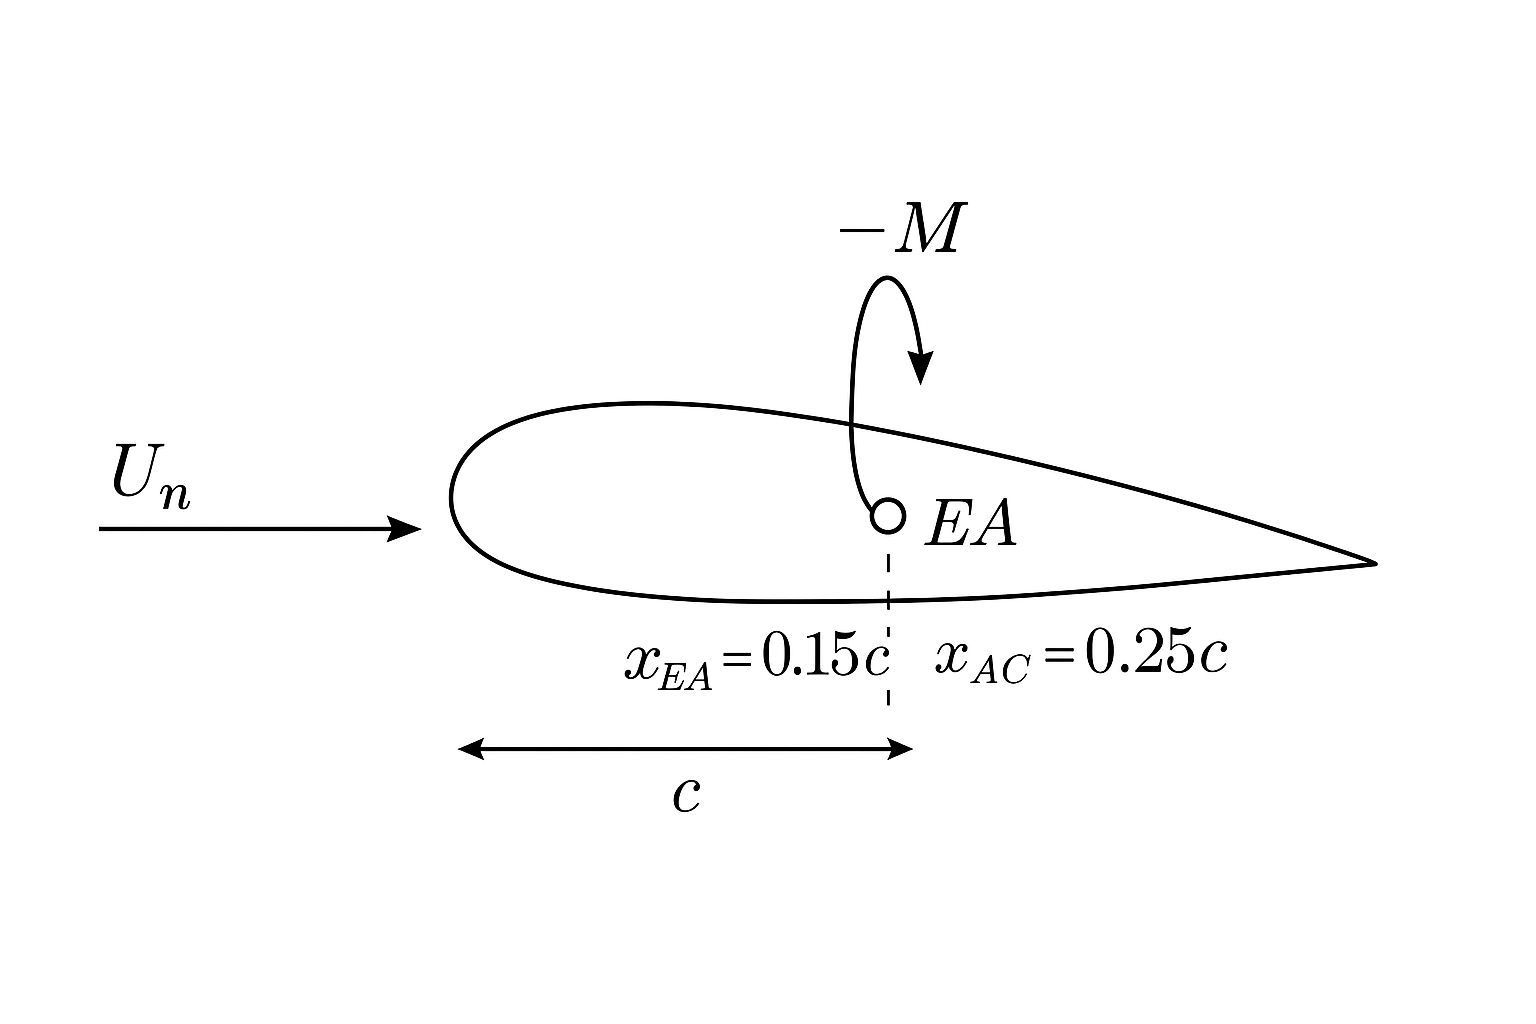
\includegraphics[width=0.75\textwidth]{fluid structure interaction.png}
\end{center}

\subsection*{Given Parameters}

\begin{itemize}
    \item Structural stiffness: \( k = 10 \, \text{Nm/rad} \)
    \item Chord length: \( c = 0.5 \, \text{m} \)
    \item Air density: \( \rho = 1.225 \, \text{kg/m}^3 \)
    \item Elastic axis location: \( x_{EA} = 0.15c \)
    \item Aerodynamic center location: \( x_{AC} = 0.25c \)
\end{itemize}

\section*{Part A: Divergence Speed Calculation}

The divergence speed \( U_{\text{div}} \) is given by:

\[
U_{\text{div}} = \sqrt{ \frac{k}{\left( \frac{1}{2} \rho c \right)(2\pi)(x_{EA} - x_{AC})} }
\]

First, compute the difference in positions:

\[
x_{EA} - x_{AC} = 0.15c - 0.25c = -0.10c = -0.10 \times 0.5 = -0.05 \, \text{m}
\]

Now substitute into the equation:

\[
U_{\text{div}} = \sqrt{ \frac{10}{\left( \frac{1}{2} \times 1.225 \times 0.5 \right)(2\pi)(-0.05)} }
\]

\[
U_{\text{div}} = \sqrt{ \frac{10}{(0.30625)(6.2832)(-0.05)} } = \sqrt{ \frac{10}{-0.0962} }
\]

This result yields a negative denominator, which indicates an \textbf{imaginary speed}, i.e., \textbf{divergence is already happening or inevitable}, because the elastic axis is in front of the aerodynamic center (\( x_{EA} < x_{AC} \)), leading to a destabilizing aerodynamic moment.

\section*{Interpretation}

When the elastic axis is located \textit{ahead} of the aerodynamic center, the aerodynamic forces effectively reduce the system stiffness. In this case, the effective stiffness becomes negative, implying instability --- the system is already beyond the divergence threshold.

\section*{Alternative: Place EA Behind AC}

To ensure divergence does not occur, the elastic axis must be behind the aerodynamic center. If instead:

\[
x_{EA} = 0.35c \quad \Rightarrow \quad x_{EA} - x_{AC} = 0.10c = 0.05 \, \text{m}
\]

Now the divergence speed becomes:

\[
U_{\text{div}} = \sqrt{ \frac{10}{(0.30625)(6.2832)(0.05)} } = \sqrt{ \frac{10}{0.0962} } \approx \sqrt{104} \approx 10.2 \, \text{m/s}
\]

\textbf{Conclusion:} For stability, the elastic axis should be placed downstream of the aerodynamic center.

\section*{Part B: Instantaneous Aerodynamic Moment}

We can calculate the instantaneous aerodynamic moment using the lift-based pitching moment formula:

\[
M = \left( \frac{1}{2} \rho U_\infty^2 c \right)(2\pi \alpha)(x_{EA} - x_{AC})
\]

Assume the following additional parameters:
\begin{itemize}
    \item Freestream velocity: \( U_\infty = 12 \, \text{m/s} \)
    \item Instantaneous angle of attack: \( \alpha = 5^\circ = 0.0873 \, \text{rad} \)
\end{itemize}

Now compute the moment:

\[
M = \left( \frac{1}{2} \cdot 1.225 \cdot 12^2 \cdot 0.5 \right)(2\pi \cdot 0.0873)(0.15c - 0.25c)
\]

\[
= (44.1)(0.548)(-0.05) \approx -1.21 \, \text{Nm}
\]

The negative sign indicates that the aerodynamic moment acts to destabilize the structure (pitches it further), consistent with earlier conclusions.

\section*{Part C: Energy Transfer via Dynamic Oscillation}

To evaluate whether energy is being added to or removed from the structure, we compute the net power transferred over one oscillation cycle:

\[
P = \frac{1}{T} \int_0^T M(t) \dot{\alpha}(t) \, dt
\]

Assume that \( M(t) \) and \( \alpha(t) \) are sinusoidal and that the hysteresis loop \( M(\alpha) \) is approximately elliptical with area \( A \approx 0.4 \, \text{Nm} \cdot \text{rad} \). Then, the average power is approximately:

\[
P \approx \frac{A}{T}
\]

Assuming \( T = 1 \, \text{s} \), we get:

\[
P \approx 0.4 \, \text{W}
\]

\textbf{Interpretation:} Since the loop is counterclockwise (as in Figure~5.45), the power is being transferred \textit{from the airfoil to the fluid}. This corresponds to damping behavior.

\section*{Final Remarks}

This extended problem illustrates the multiple layers of aeroelastic behavior:
\begin{itemize}
    \item Static instability through divergence (Part A),
    \item Time-varying aerodynamic moment (Part B),
    \item Energetic interaction and damping/amplification via power transfer (Part C).
\end{itemize}

This framework can be generalized to other configurations, such as wings with plunge degrees of freedom or spanwise flexible appendages.


\end{document}
